\documentclass[11pt, oneside]{article} 
\usepackage{geometry}
\geometry{letterpaper} 
\usepackage{graphicx}
	
\usepackage{amssymb}
\usepackage{amsmath}
\usepackage{parskip}
\usepackage{color}
\usepackage{hyperref}

\graphicspath{{/Users/telliott_admin/Tex/png/}}
% \begin{center} 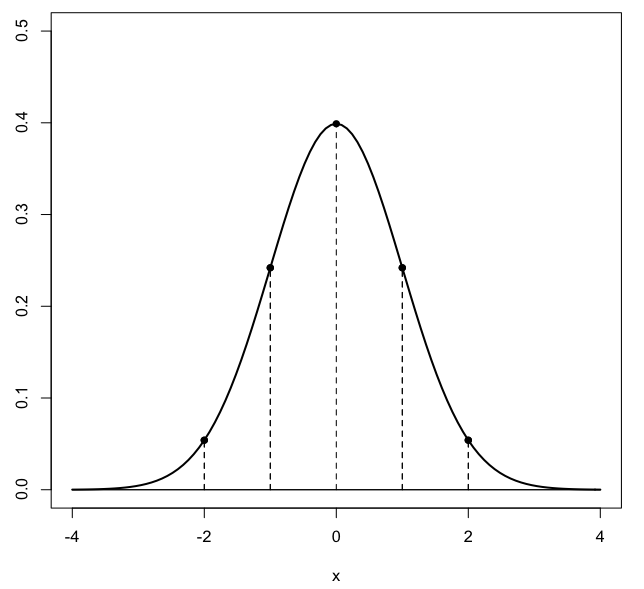
\includegraphics [scale=0.4] {gauss3.png} \end{center}

\title{Archimedes}
\date{}

\begin{document}
\maketitle
\Large


\subsection*{volume of the sphere:  geometry}
The very first derivation of the volume of a sphere was discovered by Archimedes.
The following is his "simple" but subtle argument.  

We compare a half-sphere and an inverted cone to a cylinder.  
\begin{center} 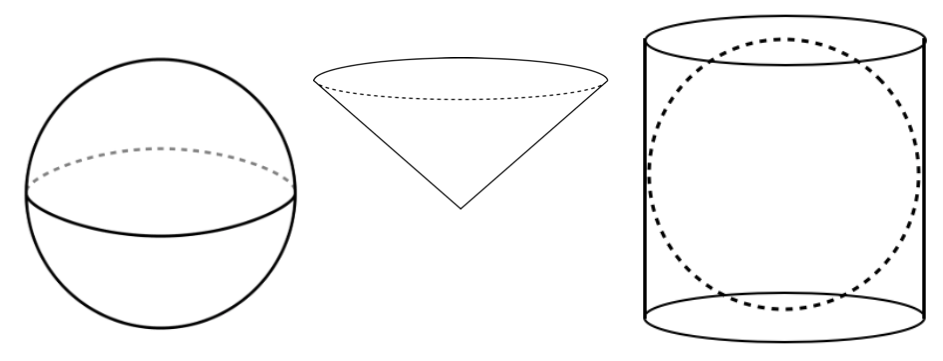
\includegraphics [scale=0.4] {scc1.png} \end{center}

Below is a diagram showing a vertical cross-section through the center of each solid so we can visualize the geometry.  The radius $R$ is the same for all three.  In addition, the cone has overall height equal to $R$.
\begin{center} 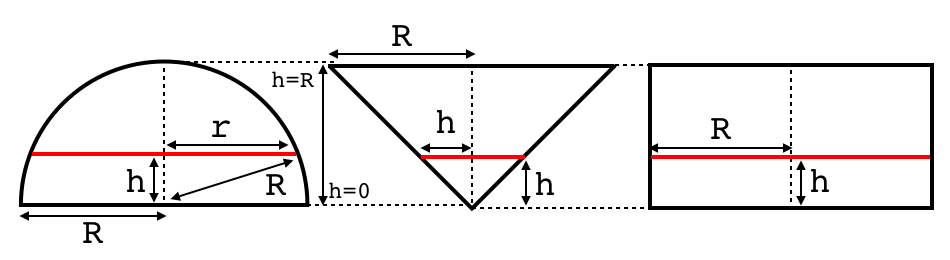
\includegraphics [scale=0.45] {scc2.png} \end{center}

Now we imagine making a horizontal slice through each solid at a height $h$, shown by the red lines.  We will choose different values of $h$ later and compare the results, the one shown here is arbitrary.

If you visualize this you should be able to see that each of these red slices is actually a circle.  Any cross-section of a sphere is a circle.  For the cylinder and cone, cross-sections perpendicular to the axis are circles as well.  

The question we ask is:  \textbf{what is the area for each horizontal slice}?

We need to determine the radius for each red circle.  Moving right-to-left, the radius of the cylinder is just $R$.  For the cone, the radius at each height $h$ is equal to $h$ (by similar triangles).  And for the sphere, we use the Pythagorean theorem to find that
\[ r^2 + h^2 = R^2 \]
\[ r^2 = R^2 - h^2 \]

For more on this theorem see \hyperref[sec:pythagorean_thm]{\textbf{here}}.

The first insight of the proof is to recognize that the radius squared for the sphere's slice ($r^2$), plus the radius squared for the cone ($h^2$) is equal to $R^2$, the radius squared for the cylinder.

Since the areas are proportional to to the radius squared (namely $A = \pi r^2$ and so on) and
\[ \pi r^2 + \pi h^2 = \pi R^2 \]
So the areas add too:  \textbf{sphere plus cone equals cylinder}.

The second insight of the proof is to recognize that this property is invariant, it does not depend on which height we choose to make the slice.  The three slices obtained at any height $h$ add up like this.  So if we imagine making a bunch of slices for each solid and adding them all up to find the volume, the volumes will add too.

This idea is now called Cavalieri's principle, though it was called the "method of indivisibles" before that.

The volume of the cylinder is simply $\pi R^3$.  The volume of the cone is known to be one-third the area of the base times the height, or $1/3 \ \pi R^3$.  (See later for a derivation).

We subtract to find that the area of the half-sphere is $2/3 \ \pi R^3$, and therefore the volume of the whole sphere is
\[ V_{\text{sphere}} = \frac{4}{3} \pi R^3 \]

There is a bit of a trick here to hide the idea introduced in calculus, which makes this thinking rigorous.  The sphere and cone have variable widths, which means that the radius will be different on the top of a slice compared to the bottom.  Therefore, the slices have to be made very thin.  In calculus they become infinitely thin, but we add up infinitely many of them.

Perhaps most interesting, Archimedes said that he discovered the correct result by balancing the three objects on a fulcrum.  

According to Archimedes (in the Method, translation by Heath)

\begin{quote}For certain things which first became clear to me by a mechanical method had afterward to be demonstrated by geometry...\textcolor{blue}{it is of course easier, when we have previously acquired by the method some knowledge of questions, to supply the proof than it is to find the proof without any previous knowledge.} This is a reason why, in the case of the theorems the proof of which Eudoxus was the first to discover, namely, that the cone is a third part of the cylinder, and the pyramid a third part of the prism, having the same base and equal height, we should give no small share of the credit to Democritus, who was the first to assert this truth...though he did not prove it.
\end{quote}

I read somewhere that what Archimedes actually balanced is a set-up like that shown here
\begin{center} 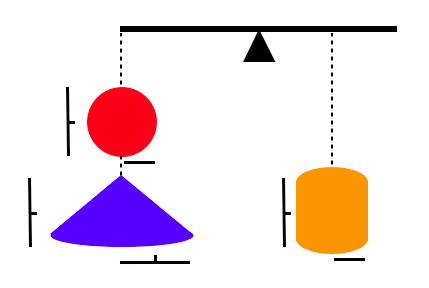
\includegraphics [scale=0.4] {archimedes1.png} \end{center}

There are three factors that complicate our calculation:  (i) we now have a single cone with radius $2r$ and height $2r$ (because it's doubled in both radius and height the cone's volume is increased by a factor of $2^3$), (ii) the sphere and cone are twice as far from the fulcrum as the cylinder, and (iii) the cylinder is made out of something denser than the other objects (four times more dense).

Let $\pi r^3$ be one unit of volume, then the volumes are

\[ \text{sphere } =   \frac{4}{3} \]
\[ \text{cone } =     \frac{1}{3} \times 8 = \frac{8}{3} \]
\[ \text{cylinder } = 2 \]

That's $12/3 = 4$ for the sphere plus cone, and furthermore they count double since they are twice the distance from the fulcrum, giving $8$ in our volume units.  So the left side is $4 \times$ the weight on the right side.  However, we are told that the density of the material for the cylinder was four times that of the objects on the left.  Hence, it should all balance.

I looked up some densities to try to guess what Archimedes used:

\begin{center}
  \begin{tabular}{ | l | l | } \hline
   marble  & $2.56$ \\ \hline
   sand & $2.80$  \\ \hline
   copper     & $8.63$  \\ \hline
   silver  & $10.40$ \\ \hline
   gold     & $19.30$  \\ \hline  
   \end{tabular}
\end{center}

How about marble and silver?

\end{document}